%%%%%%%%%%%%%%%%%%%%%%%%%%%%%%%%%%%%%%%%%
% Short Sectioned Assignment
% LaTeX Template
% Version 1.0 (5/5/12)
%
% This template has been downloaded from:
% http://www.LaTeXTemplates.com
%
% Original author:
% Frits Wenneker (http://www.howtotex.com)
%
% License:
% CC BY-NC-SA 3.0 (http://creativecommons.org/licenses/by-nc-sa/3.0/)
%
% Download template:
% Overleaf (https://www.overleaf.com/8746855dtrgkbkbjjhm)
%
%%%%%%%%%%%%%%%%%%%%%%%%%%%%%%%%%%%%%%%%%

%-------------------------------------------------------------------------------
%	PACKAGES AND OTHER DOCUMENT CONFIGURATIONS
%-------------------------------------------------------------------------------

%\documentclass[paper=a4, fontsize=11pt]{scrartcl} % A4 paper and 11pt font size
\documentclass[a4paper]{article}

%\usepackage[options]{nohyperref}  % This makes hyperref commands do nothing without errors
%\usepackage{url}  % This makes \url work
%\usepackage{hyperref}

\usepackage{graphicx}

%\usepackage[T1]{fontenc} % Use 8-bit encoding that has 256 glyphs
\usepackage[utf8]{inputenc}
%\usepackage{fourier} % Use the Adobe Utopia font for the document - comment this line to return to the LaTeX default
\usepackage[english]{babel} % English language/hyphenation
\usepackage{amsmath,amsfonts,amsthm} % Math packages

%\usepackage{lipsum} % Used for inserting dummy 'Lorem ipsum' text into the template

\usepackage{sectsty} % Allows customizing section commands
\allsectionsfont{\centering \normalfont\scshape} % Make all sections centered, the default font and small caps

\usepackage{fancyhdr} % Custom headers and footers
\pagestyle{fancyplain} % Makes all pages in the document conform to the custom headers and footers
\fancyhead{} % No page header - if you want one, create it in the same way as the footers below
\fancyfoot[L]{} % Empty left footer
\fancyfoot[C]{} % Empty center footer
\fancyfoot[R]{\thepage} % Page numbering for right footer
\renewcommand{\headrulewidth}{0pt} % Remove header underlines
\renewcommand{\footrulewidth}{0pt} % Remove footer underlines
\setlength{\headheight}{13.6pt} % Customize the height of the header

\numberwithin{equation}{section} % Number equations within sections (i.e. 1.1, 1.2, 2.1, 2.2 instead of 1, 2, 3, 4)
\numberwithin{figure}{section} % Number figures within sections (i.e. 1.1, 1.2, 2.1, 2.2 instead of 1, 2, 3, 4)
\numberwithin{table}{section} % Number tables within sections (i.e. 1.1, 1.2, 2.1, 2.2 instead of 1, 2, 3, 4)

%\setlength\parindent{0pt} % Removes all indentation from paragraphs - comment this line for an assignment with lots of text
\usepackage{indentfirst} % Indentation for all paragraphs

% Used for definitions:
\usepackage{amsthm}
\theoremstyle{definition}
\newtheorem{definition}{Definition}[section]

% To write algorithms in pseudocode:
\usepackage{algpseudocode}
\usepackage{algorithm}

% Don't use colon in algorithms lines:
\algrenewcommand\alglinenumber[1]{\footnotesize #1}

% Input/Output instead of Require/Ensure in algorithms pseudocode:
\renewcommand{\algorithmicrequire}{\textbf{Input:}}
\renewcommand{\algorithmicensure}{\textbf{Output:}}

% To put images side by side:
\usepackage{subcaption}

%-------------------------------------------------------------------------------
%	TITLE SECTION
%-------------------------------------------------------------------------------

\newcommand{\horrule}[1]{\rule{\linewidth}{#1}} % Create horizontal rule command with 1 argument of height

\title{
\normalfont \normalsize
\textsc{Sapienza University of Rome} \\ [25pt] % Your university, school and/or department name(s)
\horrule{0.5pt} \\[0.4cm] % Thin top horizontal rule
\huge Optimization Methods for Machine Learning \\ % The assignment title
\large Homework 1 \\
\horrule{2pt} \\[0.5cm] % Thick bottom horizontal rule
}

\author{Ivan Bergonzani, Michele Cipriano} % Your name

\date{\normalsize\today} % Today's date or a custom date

\begin{document}

\maketitle % Print the title

%-------------------------------------------------------------------------------

\section{Introduction}

The aim of the homework is to train and compare different neural networks on a
regression problem. In particular, the regression task is performed on the Franke's
function, building a dataset from it by sampling 100 random points $(x^i, y^i)$ with noise,
i.e. with $y^i = F(x^i) + \varepsilon^i$ where $\varepsilon^i$ is a random number in
$[-10^{-1}, 10^{-1}]$ and $F$ is the Franke's function.
The dataset has been split into a training set (70\% of the dataset)
and a test set (the remaining 30\%).

Two architectures have been compared using different training methods and different
hyperparameters. In particular, the multi-layer perceptron (MLP) and the radial basis
function network (RBFN) have been trained with full minimization, two blocks method
and decomposition method. In the full minimization, the training
error is minimized w.r.t all the weights using the gradient descent algorithm.
In the two blocks method, for the MLP
the error is minimized via an extreme learning procedure and for the RBFN the
error is minized by first selecting the centers through a clustering algorithm
and then by solving a linear least squares problem. In the decomposition method
the error is minimized by alternating a convex minimization w.r.t. the output
weights and a non-convex minimization w.r.t. all the other weights.

The best result has been obtained with TODO, which has an error of \textbf{TODO}
on the test set. The project has been developed in Python with TensorFlow and
Numpy for the learning algorithms and the computation of the tensors.

%-------------------------------------------------------------------------------

\section{Full Minimization}

As mentioned before, the full minimization is done by using the gradient
descent algorithm on the training error function, defined as:

\[ E(\omega; \pi) = \frac{1}{2P} \displaystyle\sum_{p=1}^{P} \| f\big(x^p\big) - y^p \|^2
+ \rho \| \omega \|^2 \]

\noindent where $\omega$ = ($v$, $w$, $b$) are the weights,
$\pi$ = ($N$, $\rho$, $\sigma$) are the hyperparameters, $P$ is the dimension
of the training set and $f$ is the function computed by the neural network.

Let's consider a shallow MLP with linear output:

\[ f(x) = \displaystyle\sum_{j=1}^{N} v_j g\left(\displaystyle\sum_{i=1}^{n}w_{ji}x_i - b_j\right) \]

\noindent with $n$ dimension of the input, $N$ dimension of hidden layer, $v \in \mathbb{R}^N$
weights from the hidden to the output layer and
$g$ activation function, defined as:

\[ g(t) = tanh\left(\frac{t}{2}\right) = \frac{1-e^{-\sigma t}}{1+e^{-\sigma t}} \]

The training has been performed over 15000 iterations on the training set with
a learning rate $\eta = 0.001$. The hyperparameters have been tuned with a
grid search over all the possible combinations of the hyperparameters in:

\[ (N, \rho, \sigma) \in \Big\{25, 50, 75, 100\Big\} \times \Big\{10^{-3}, 10^{-4}, 10^{-5}\Big\}
\times \Big\{1, 2, 3, 4\Big\} \]

\noindent selecting the network with the lowest error on the test set.
The best result obtained an error of 0.009 on the training set and an error of
0.006 on the test set as it is also possible to see in table \ref{tab:experiments}.
The hyperparameters found are $N=75$, $\rho=10^{-5}$ and $\sigma=3$. In figure \ref{fig:plots}
the plot of the function computed by the MLP found.

TODO: explain overfitting/underfitting

An analogous experiment has been done with the radial basis function network,
defined as:

\[ f(x) = \displaystyle\sum_{j=1}^{N} v_j \phi(\| x^i - c_j \|) \]

where $c_j \in \mathbb{R}^2$ is the center of the j-th hidden neuron,
$v \in \mathbb{R}^N$ weights from the hidden to the output layer and $\phi$
is the activation function, defined as:

\[ \phi(\|x - c_j\|) = e^{-(\| x - c_j \|/\sigma)^2} \]

\noindent with $\sigma > 0$.
The training has been performed over 15000 iterations on the training set with
a learning rate $\eta = 0.001$. The hyperparameters have been tuned with a
grid search over all the possible combinations of the hyperparameters in:

\[ (N, \rho, \sigma) \in \Big\{25, 50, 70\Big\} \times \Big\{10^{-3}, 10^{-4}, 10^{-5}\Big\}
\times \Big\{0.25, 0.5, 0.75, 1\Big\} \]

\noindent selecting the network with the lowest error on the test set.
The best result obtained an error of TODO on the training set and an error of
TODO on the test set (see table \ref{tab:experiments}).
The hyperparameters found are $N=0$, $\rho=0$ and $\sigma=0$. In figure \ref{fig:plots}
the plot of the function computed by the RBFN found.

As already said before, both training procedures for MLP and RBFN have been
performed using the gradient descent algorithm for 15000 iterations with a
learning rate $\eta = 0.001$. This step has been implemented with TensorFlow's
gradient descent optimizer, defined in \texttt{tf.train.GradientDescentOptimizer}.
For each hyperparameter setting the training took 0.00s for the MLP and 0.00s
for the RBFN on average.

TODO: explain overfitting/underfitting

TODO: MLP vs RBFN

%-------------------------------------------------------------------------------

\section{Two Blocks Method}

The idea, here, is to train the network by first setting up a subset of weights
and then by solving efficiently the least squares problem obtained. This
speeds up the training of the network obtaining (similar?) results w.r.t the
previous section.

For what regards the MLP all the weights $w_{ji}$ and the biases $b_j$, with
$j \in \{ 1, ..., N \} $ and $i \in \{ 1, ..., n \} $, have been set up
randomly. This reduces the minimization problem to the solution of:

\begin{equation}
 	\label{eq:min-nabla-v}
	\nabla_v E(\omega; \pi) = 0
\end{equation}

\noindent where the hyperparameters $\pi$ are the values found in the previous
section. Hence, the problem becomes a simple linear system:

\[ \left( \frac{1}{2P} G^T G + \rho I \right) v = \frac{1}{2P} G^T y \]

\noindent where $G \in \mathbb{R}^{P \times N}$ is defined as:

\[ G_{rc} = g\left( \sum_{i=1}^{n} w_{ci}x_i^r - b_c \right) \]

This method has been performed 10000 times obtaining an error of TODO on the
training set and an error of TODO on the test set (table \ref{tab:experiments}). In figure
\ref{fig:plots} the plot of the function computed by the MLP found.

TODO: COMPARISON WITH Q1E1

An analogous procedure has been applied to RBFN.
The centers $c_j$, with $ j \in \{ 1,  ..., N \} $ have been selected by
using the K-means clustering algorithm. This allowed, as before, to reduce the
problem to the solution of equation \ref{eq:min-nabla-v}. The hyperparameters
are the ones found in the previous section. Here G is defined as:

\[ G_{ij} = \phi\left( \| x^i - c_j \| \right) \]

This method has been performed 10000 times obtaining an error of TODO on the
training set and an error of TODO on the test set (table \ref{tab:experiments}). In figure
\ref{fig:plots} the plot of the function computed by the RBFN found.

TODO: COMPARISON WITH Q1E2

TODO: implementation of both MLP and RBFN

%-------------------------------------------------------------------------------

\section{Decomposition Method}

TODO: E3

%-------------------------------------------------------------------------------

\section{Conclusion}

\begin{table}
	\centering
	\begin{tabular}{*{7}{c}}
		Neural Network & N & $\sigma$ & $\rho$ & Training Error & Test Error & Time \\
		\hline
		Full MLP & 75 & 3 & $10^{-5}$ & 0.007 & 0.006 & 25.587s \\
		Full RBFN & 50 & 0.25 & $10^{-5}$ & 0.005 & 0.005 & 34.770s \\
		Extreme MLP & 75 & 3 & $10^{-5}$ & 0.002 & 0.002 & 0.001s \\
		Unsupervised c. RBFN & 50 & 0.25 & $10^{-5}$ & 0.001 & 0.003 & 0.001s \\
		TBD & TBD & TBD & TBD & TBD & \textbf{TBD} & TBD \\
	\end{tabular}
	\caption{Results of the experiments described in the previous sections.
		The last column shows the amount of time needed to train each
		specific network.}
	\label{tab:experiments}
\end{table}

Conclusion. (Remember to say that all experiments have been performed on
a kind of computer)

\begin{figure}[H]
	\centering
	\begin{subfigure}{.32\textwidth}
		\centering
		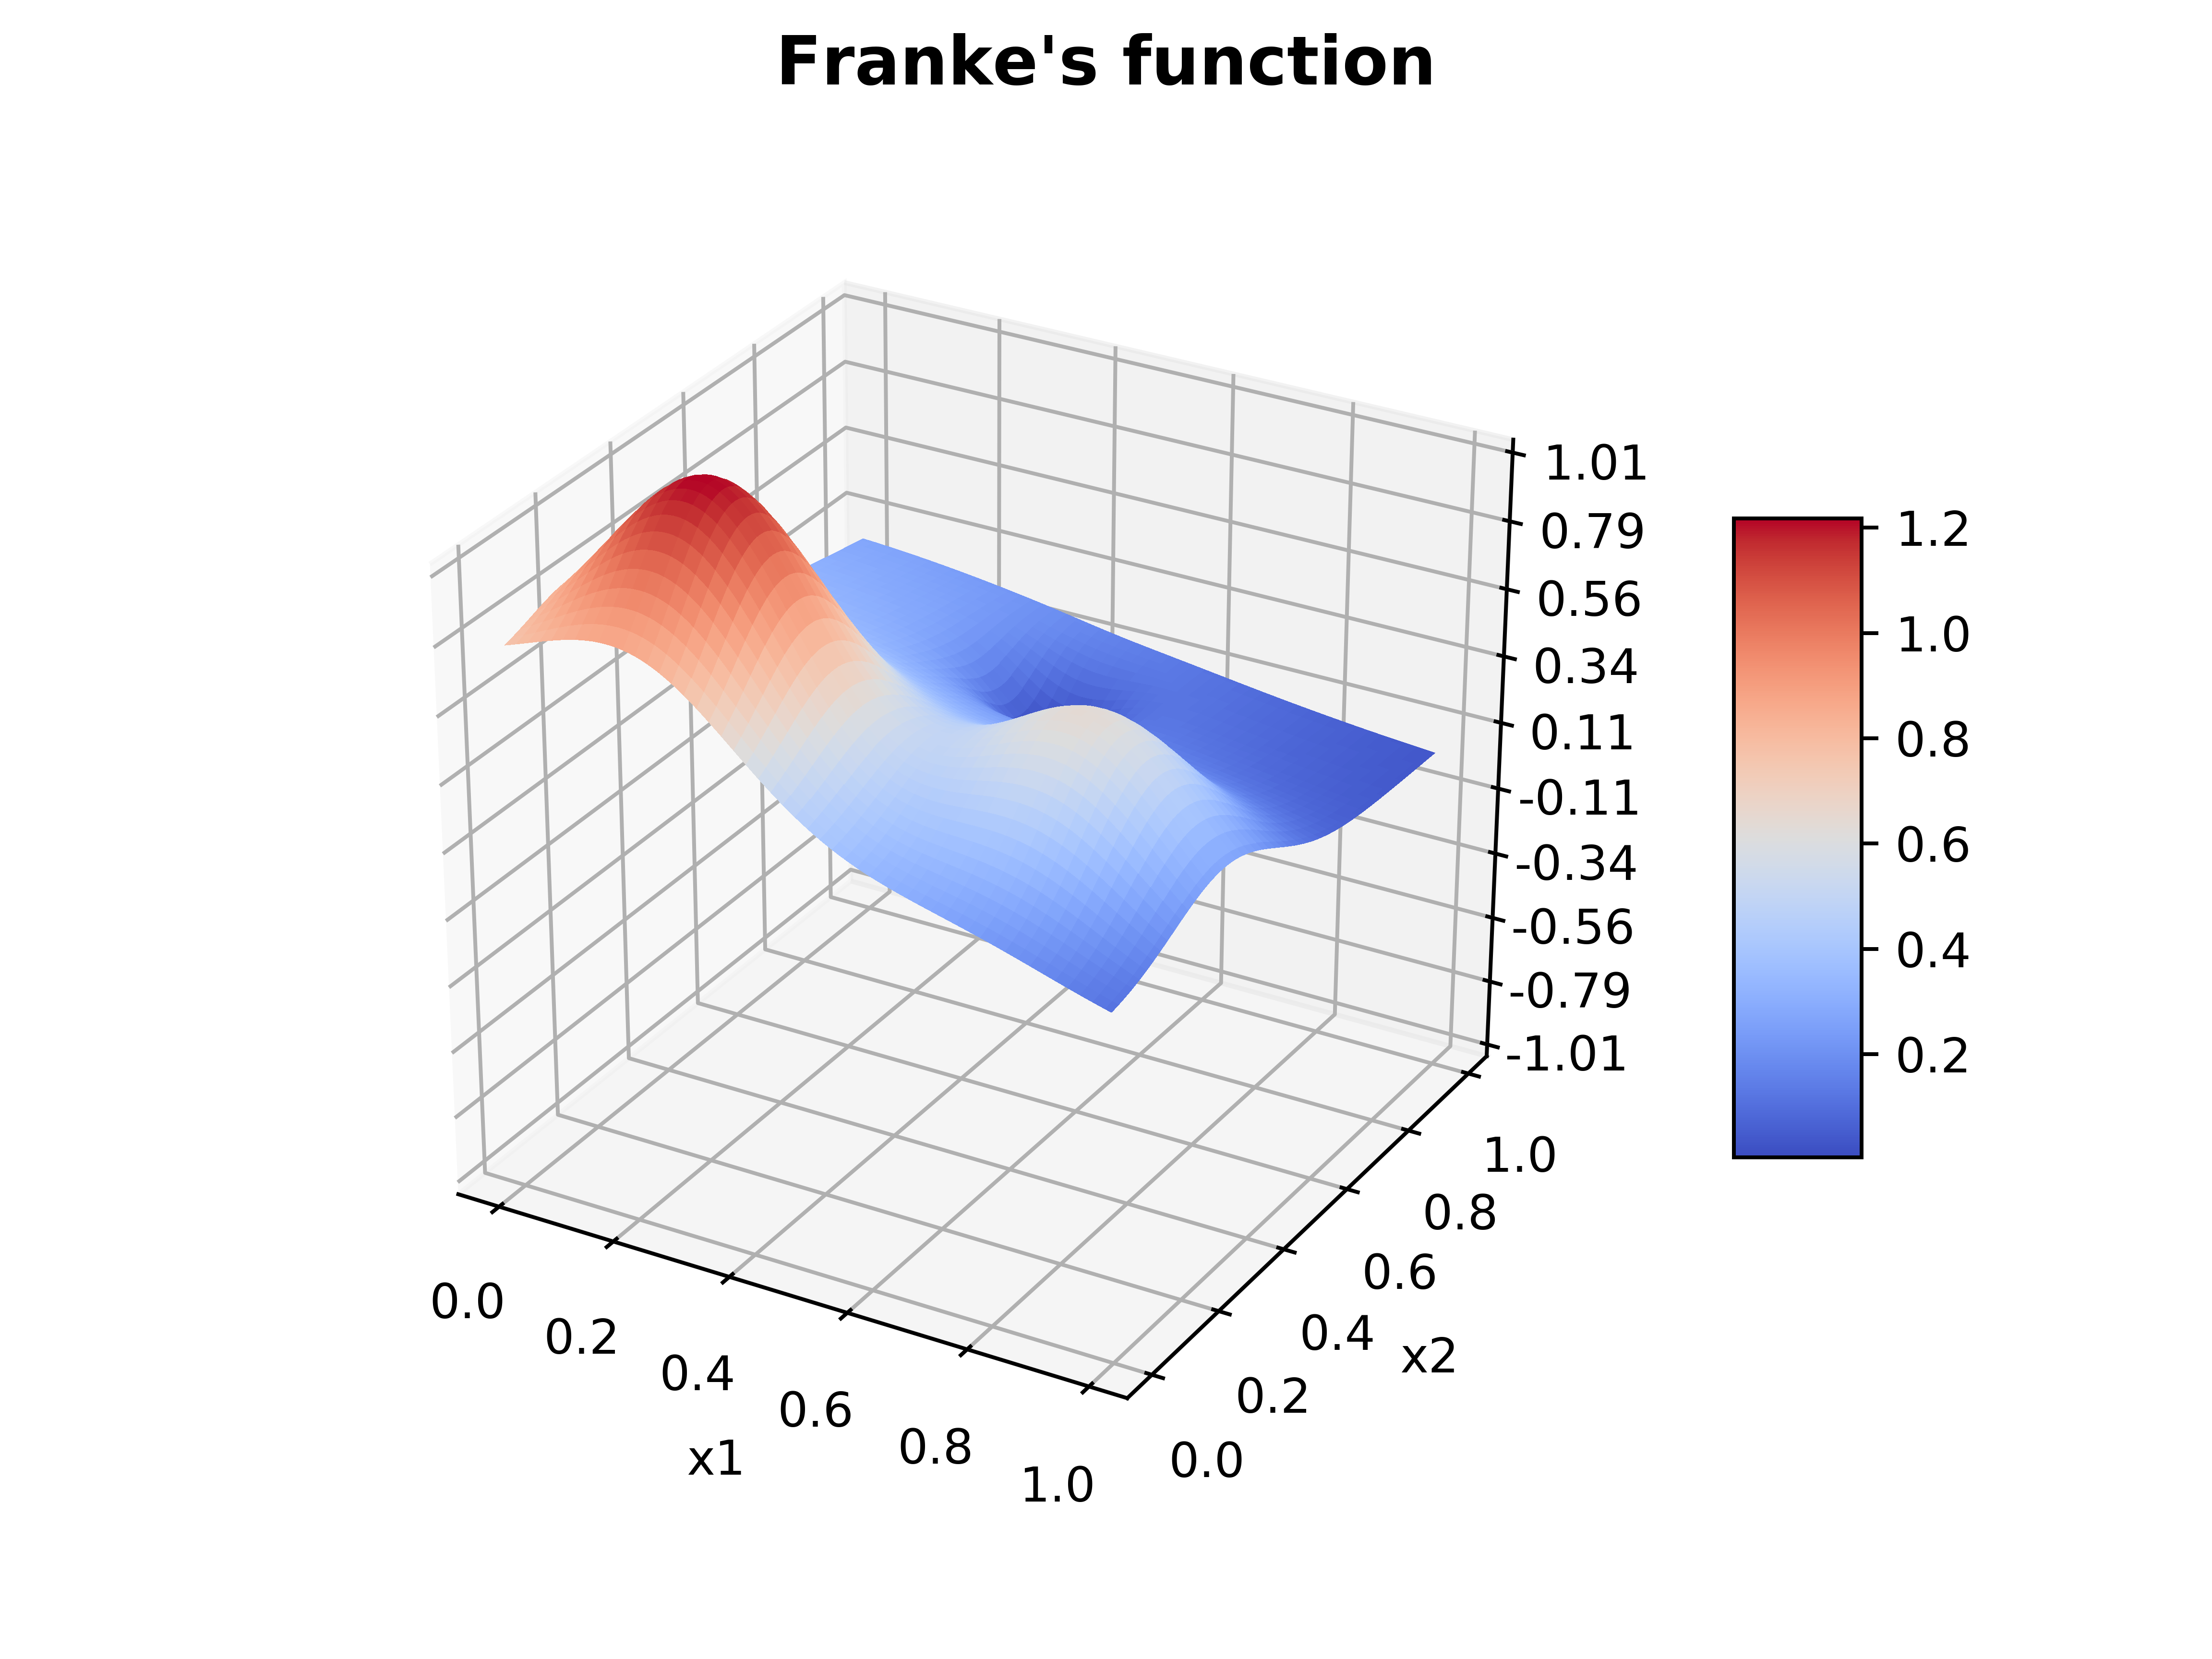
\includegraphics[width=1.0\linewidth]{images/franke.png}
	\end{subfigure}
	\begin{subfigure}{.32\textwidth}
		\centering
		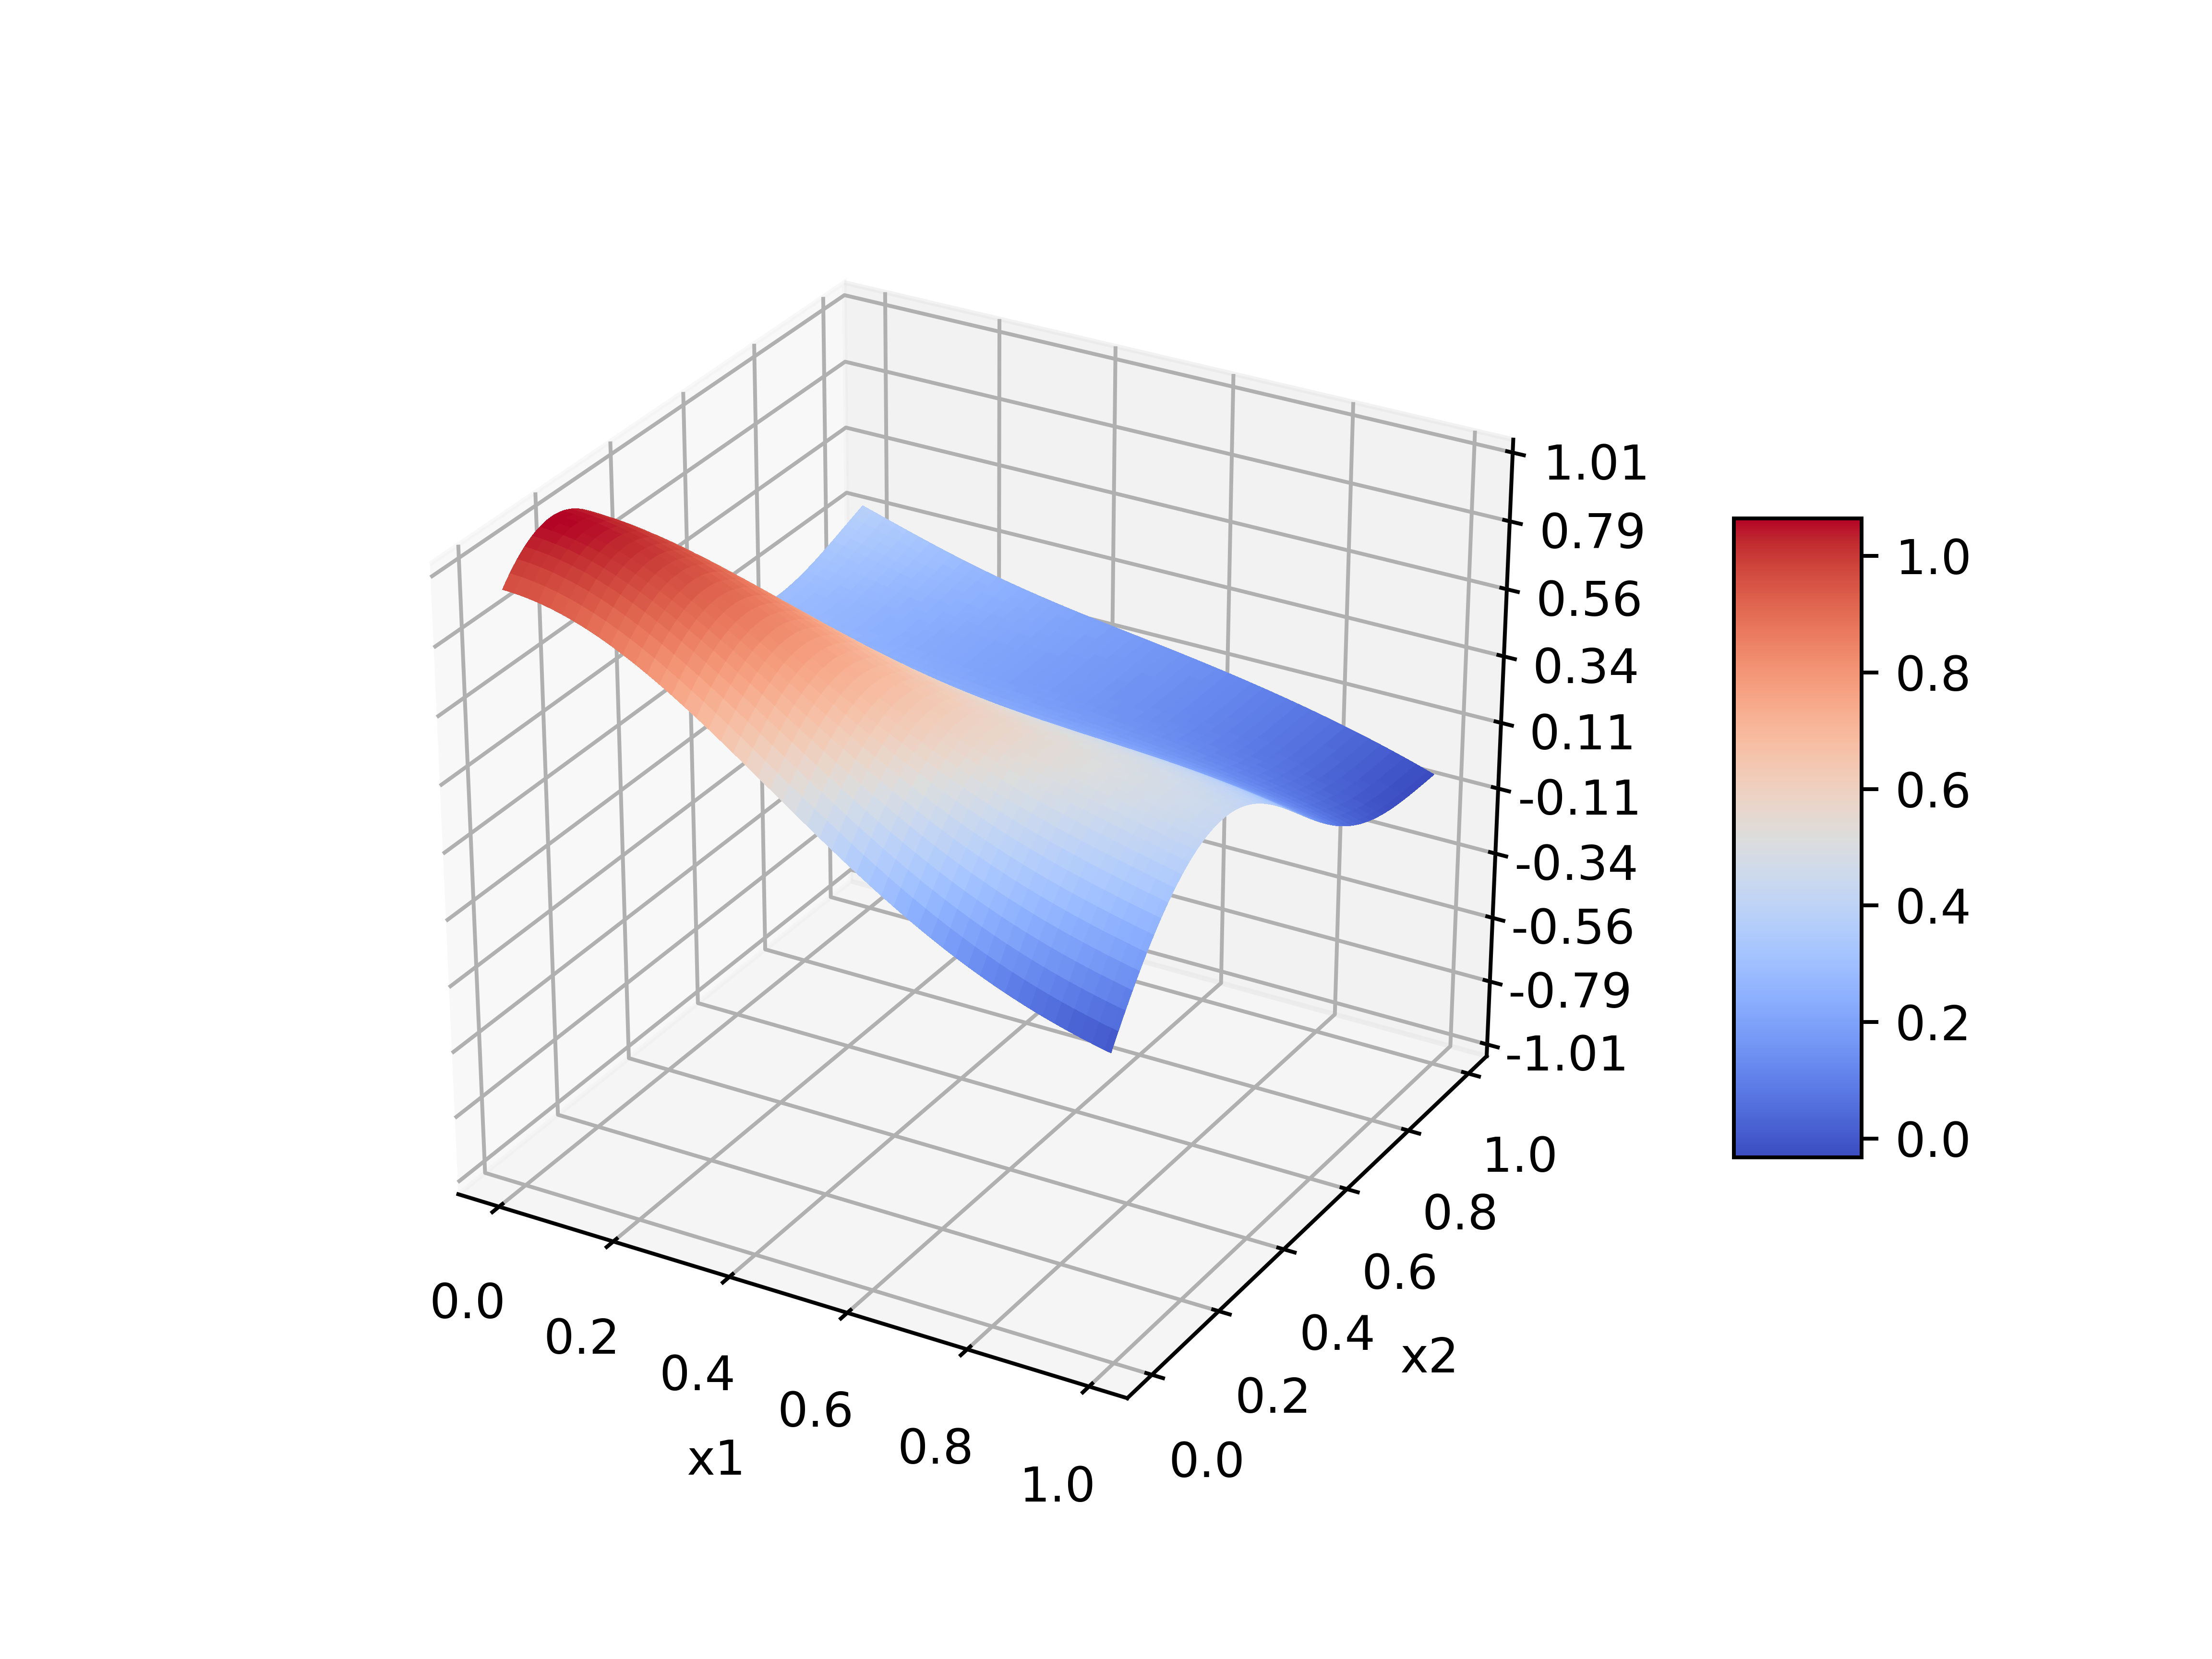
\includegraphics[width=1.0\linewidth]{images/MLP_N_75_sigma_3_rho_1e-05.png}
	\end{subfigure}
	\begin{subfigure}{.32\textwidth}
		\centering
		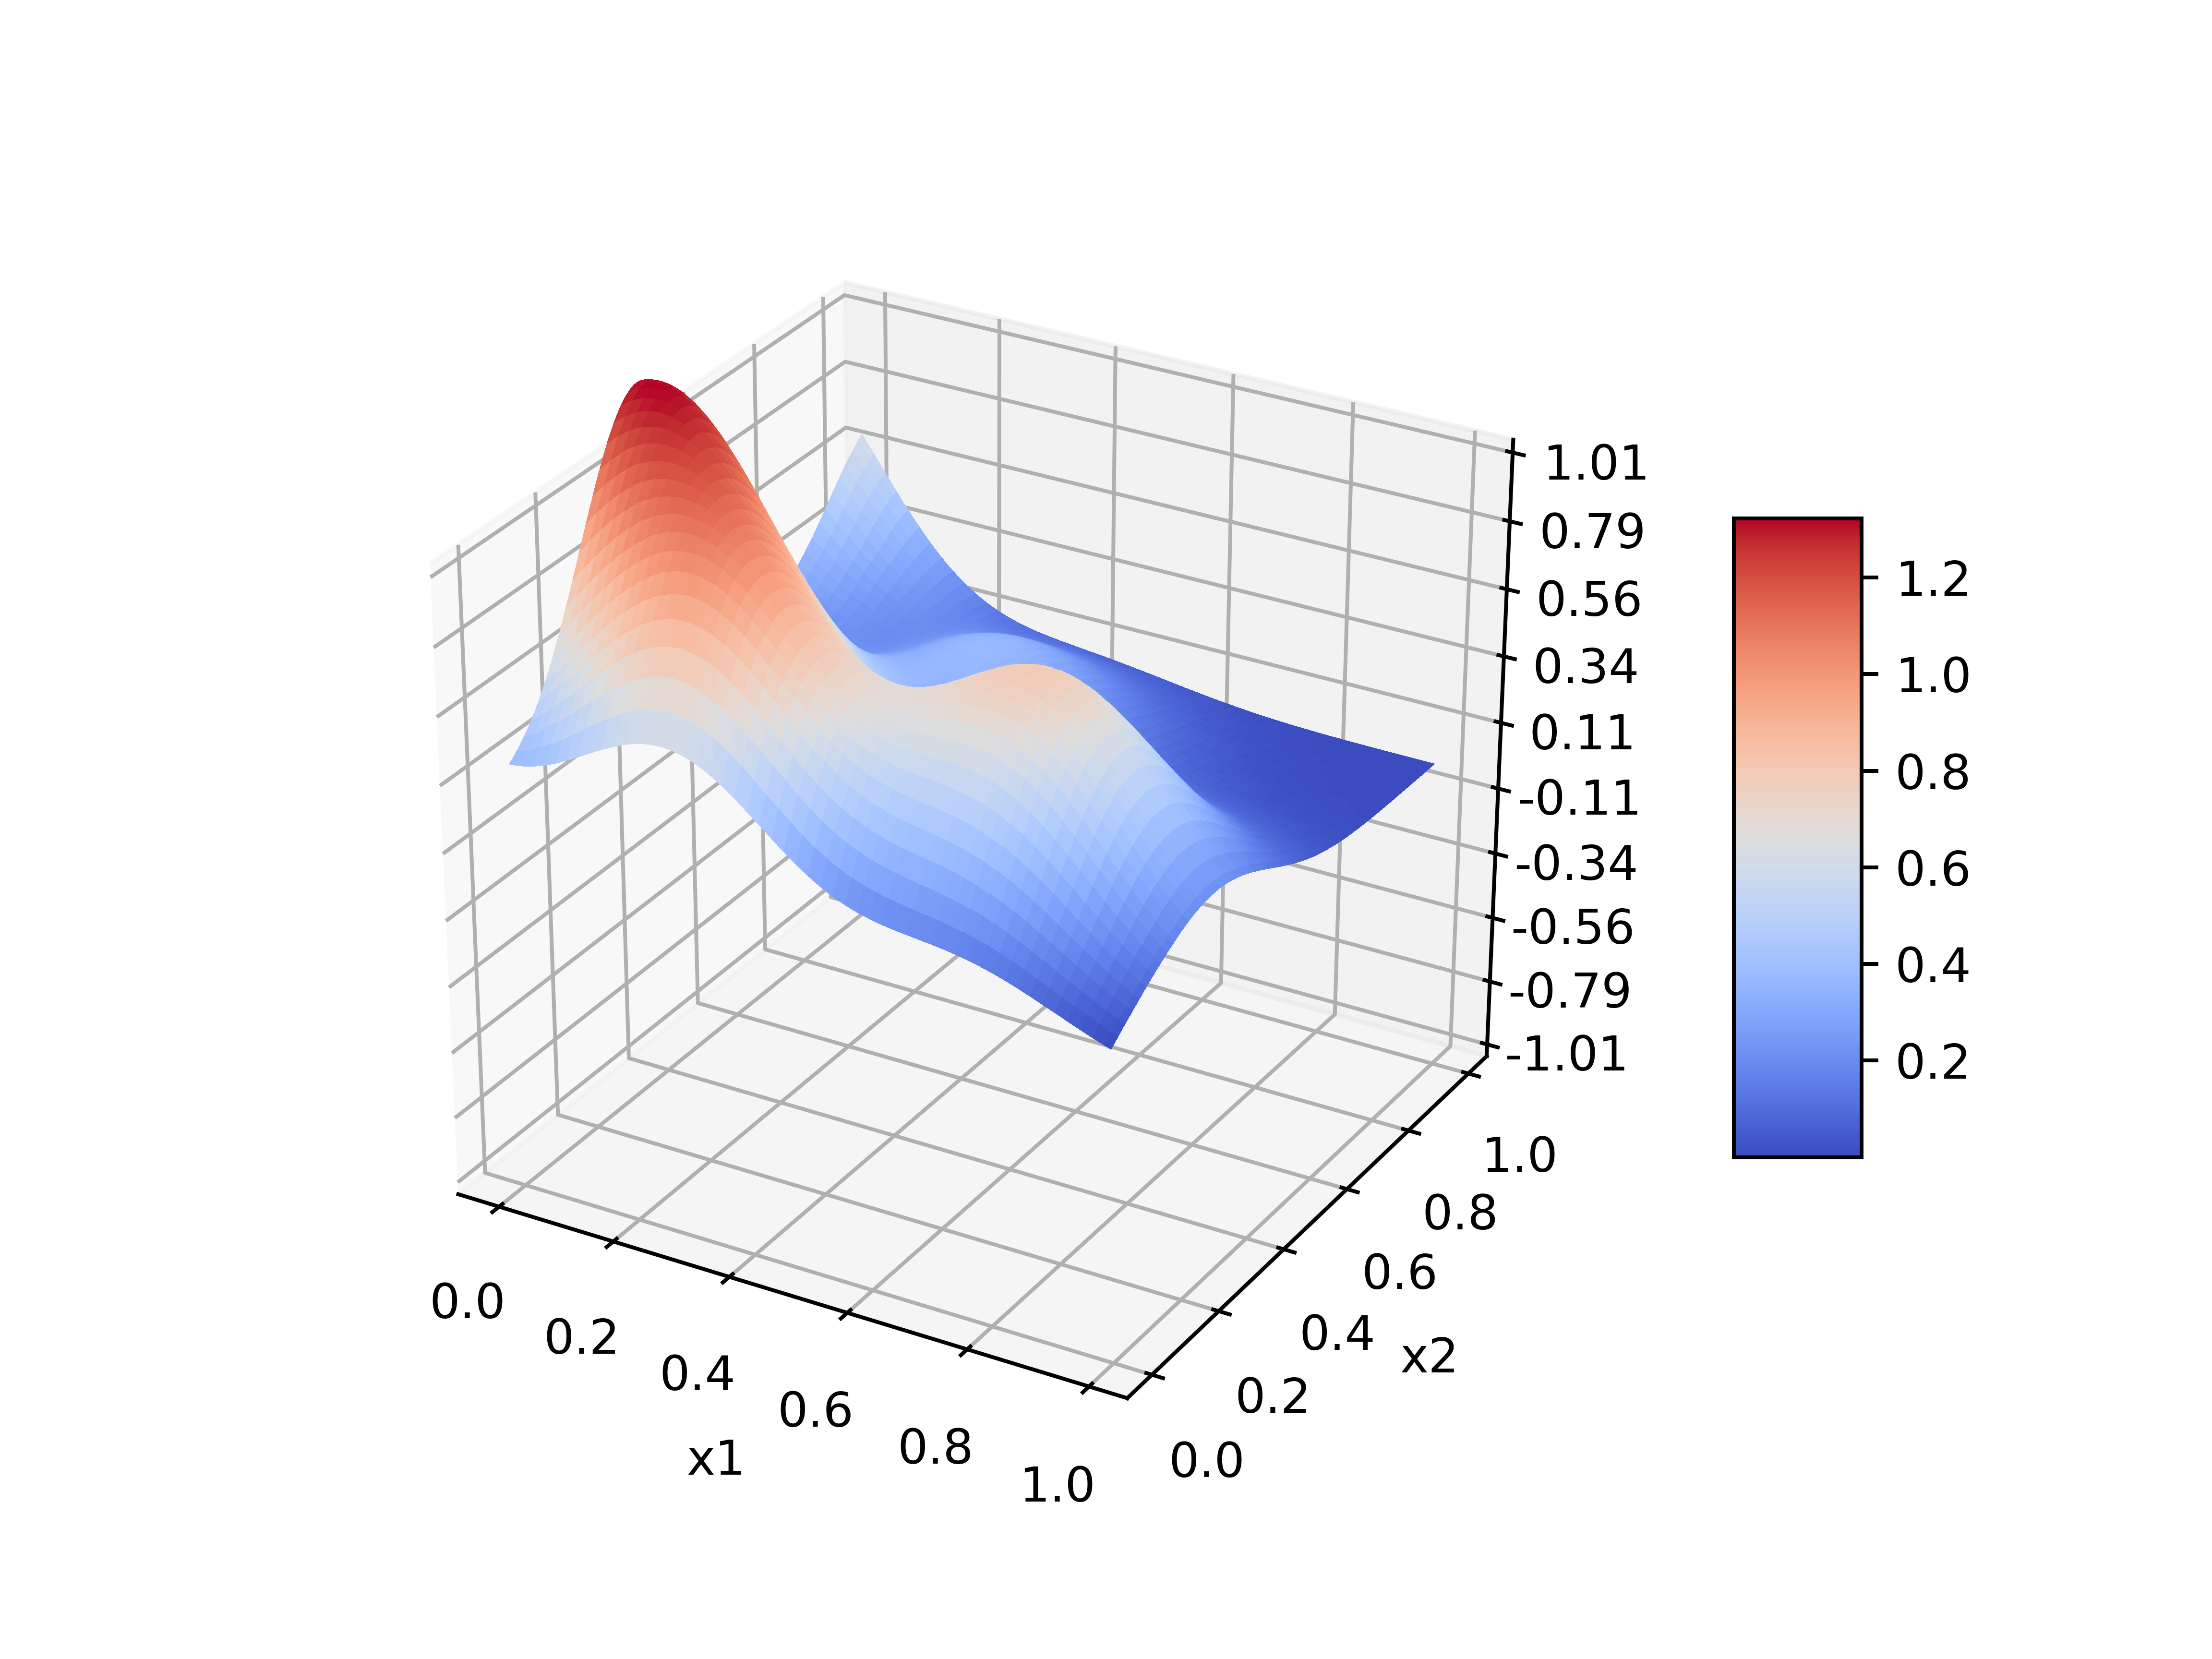
\includegraphics[width=1.0\linewidth]{images/RBFN_N_50_sigma_025_rho_00001.png}
	\end{subfigure}
	\begin{subfigure}{.32\textwidth}
		\centering
		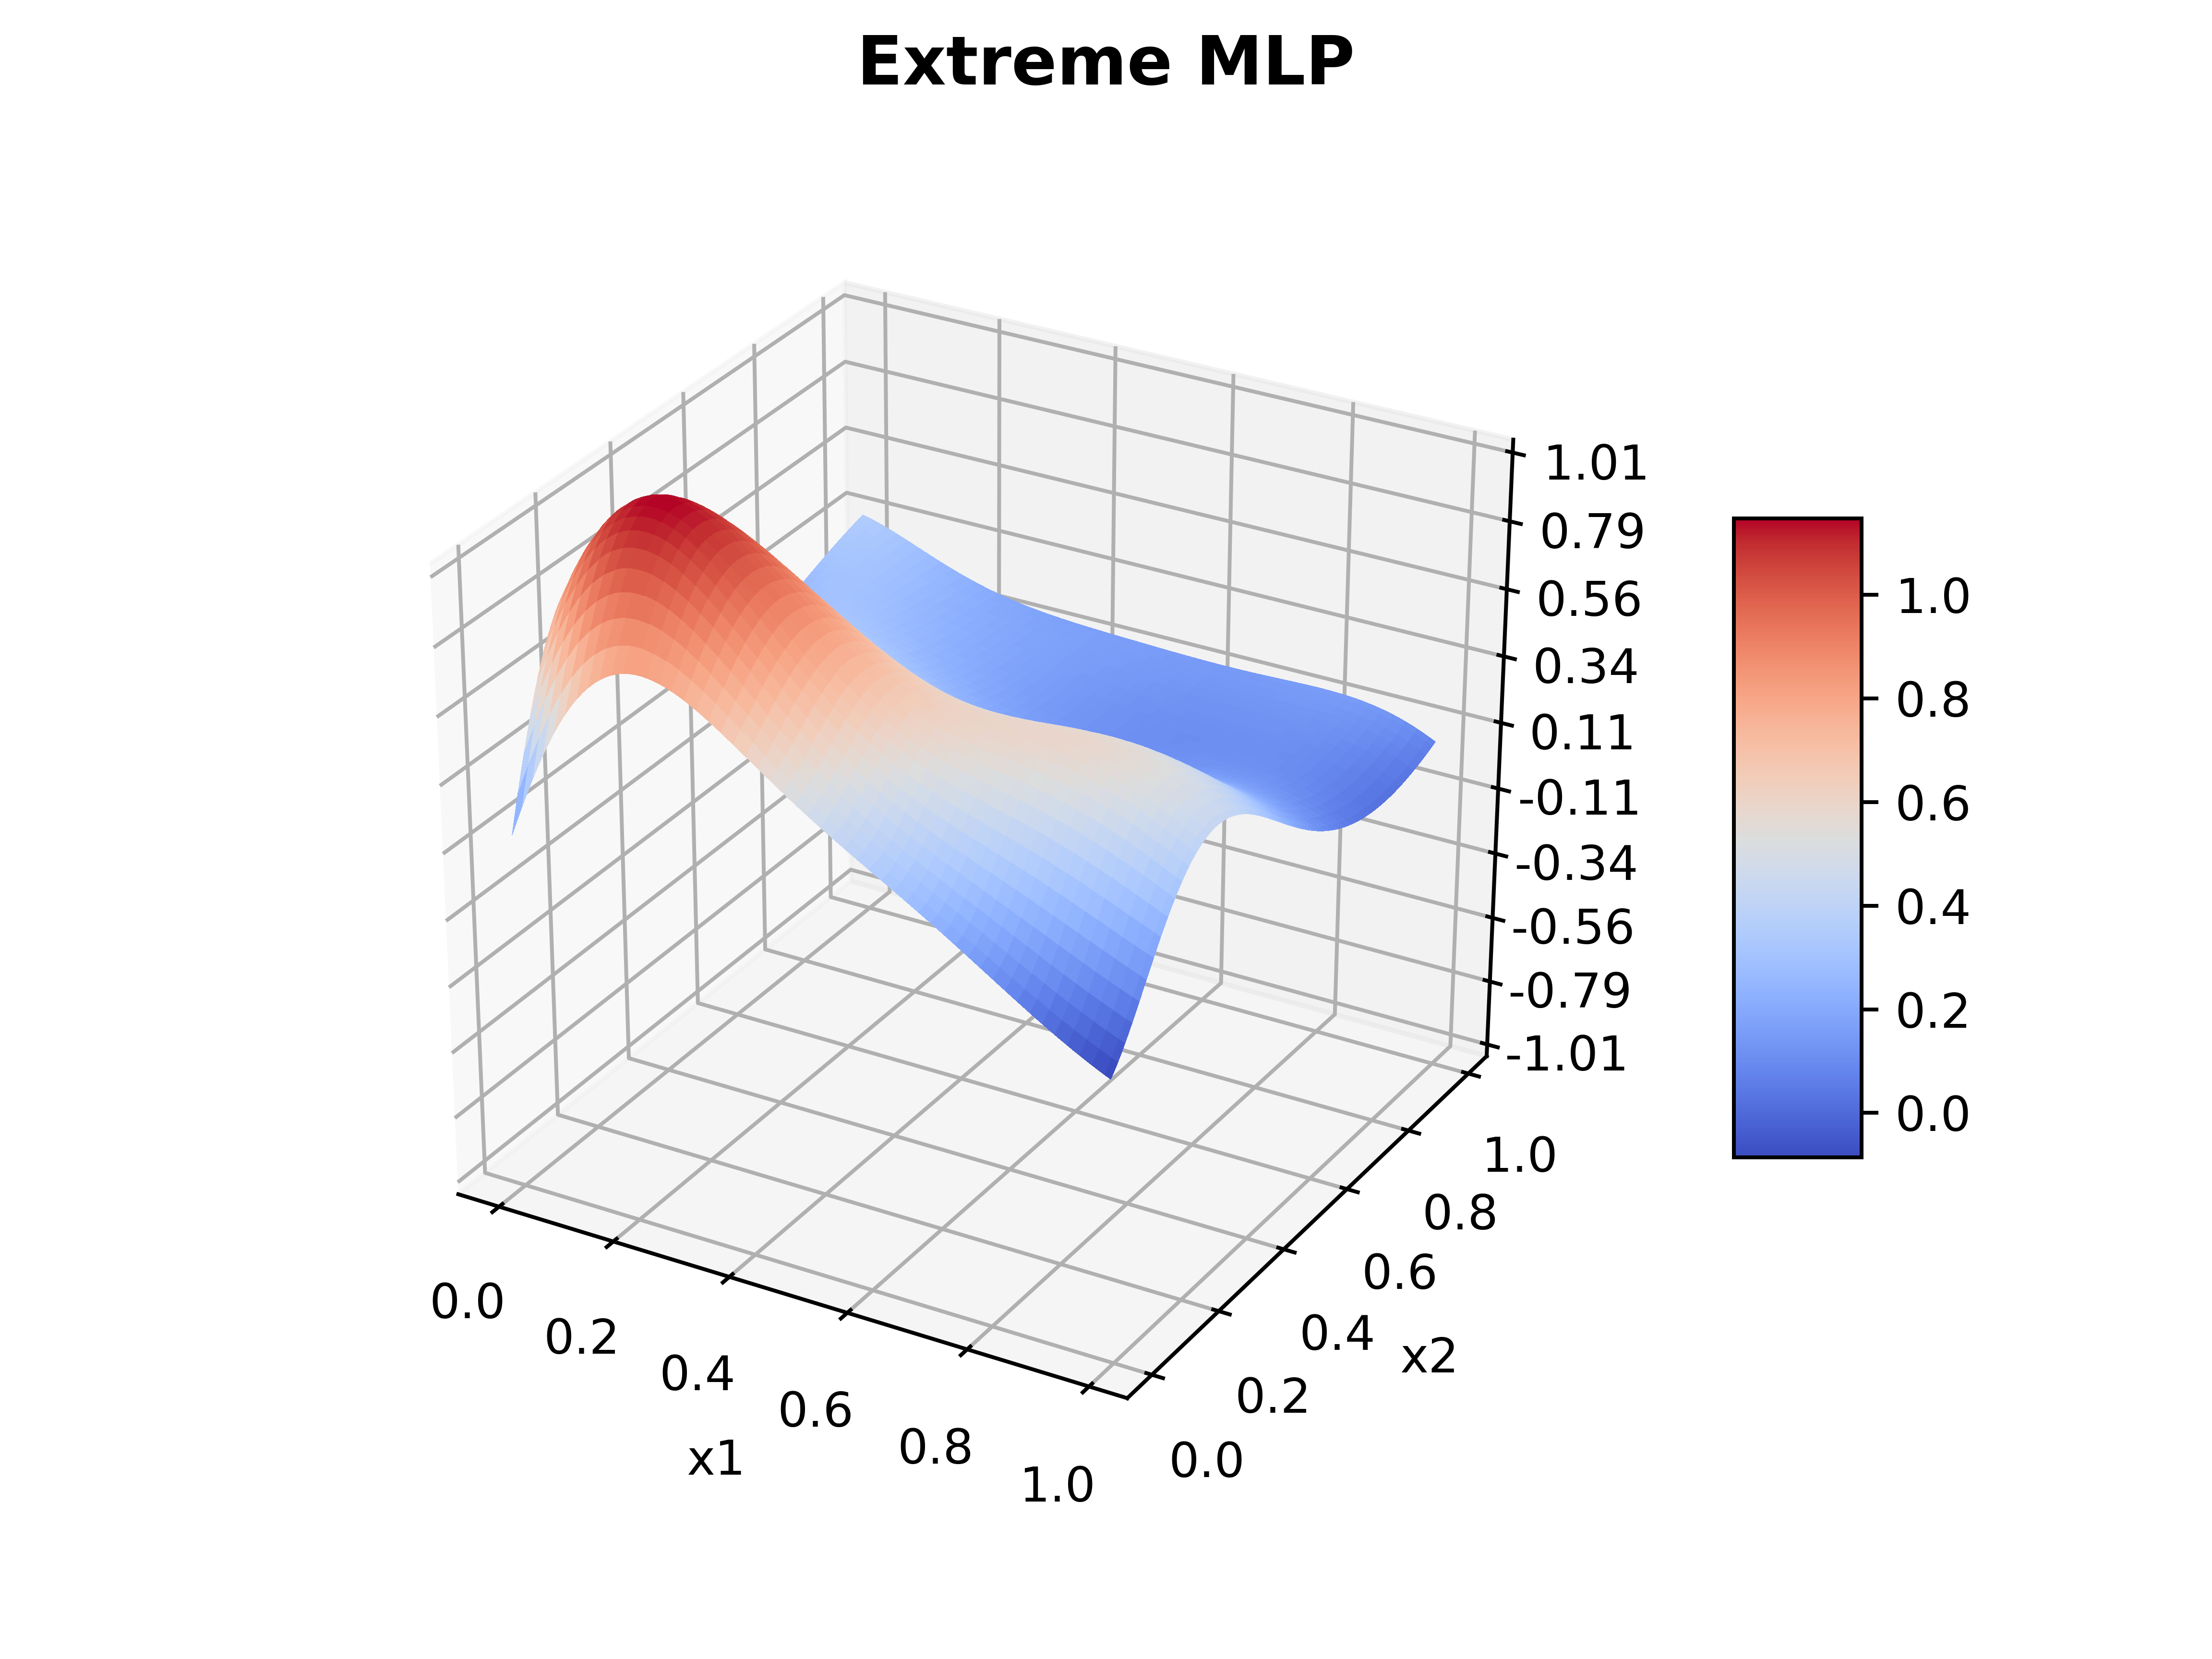
\includegraphics[width=1.0\linewidth]{images/MLP_Extreme_Learning.png}
	\end{subfigure}
	\begin{subfigure}{.32\textwidth}
		\centering
		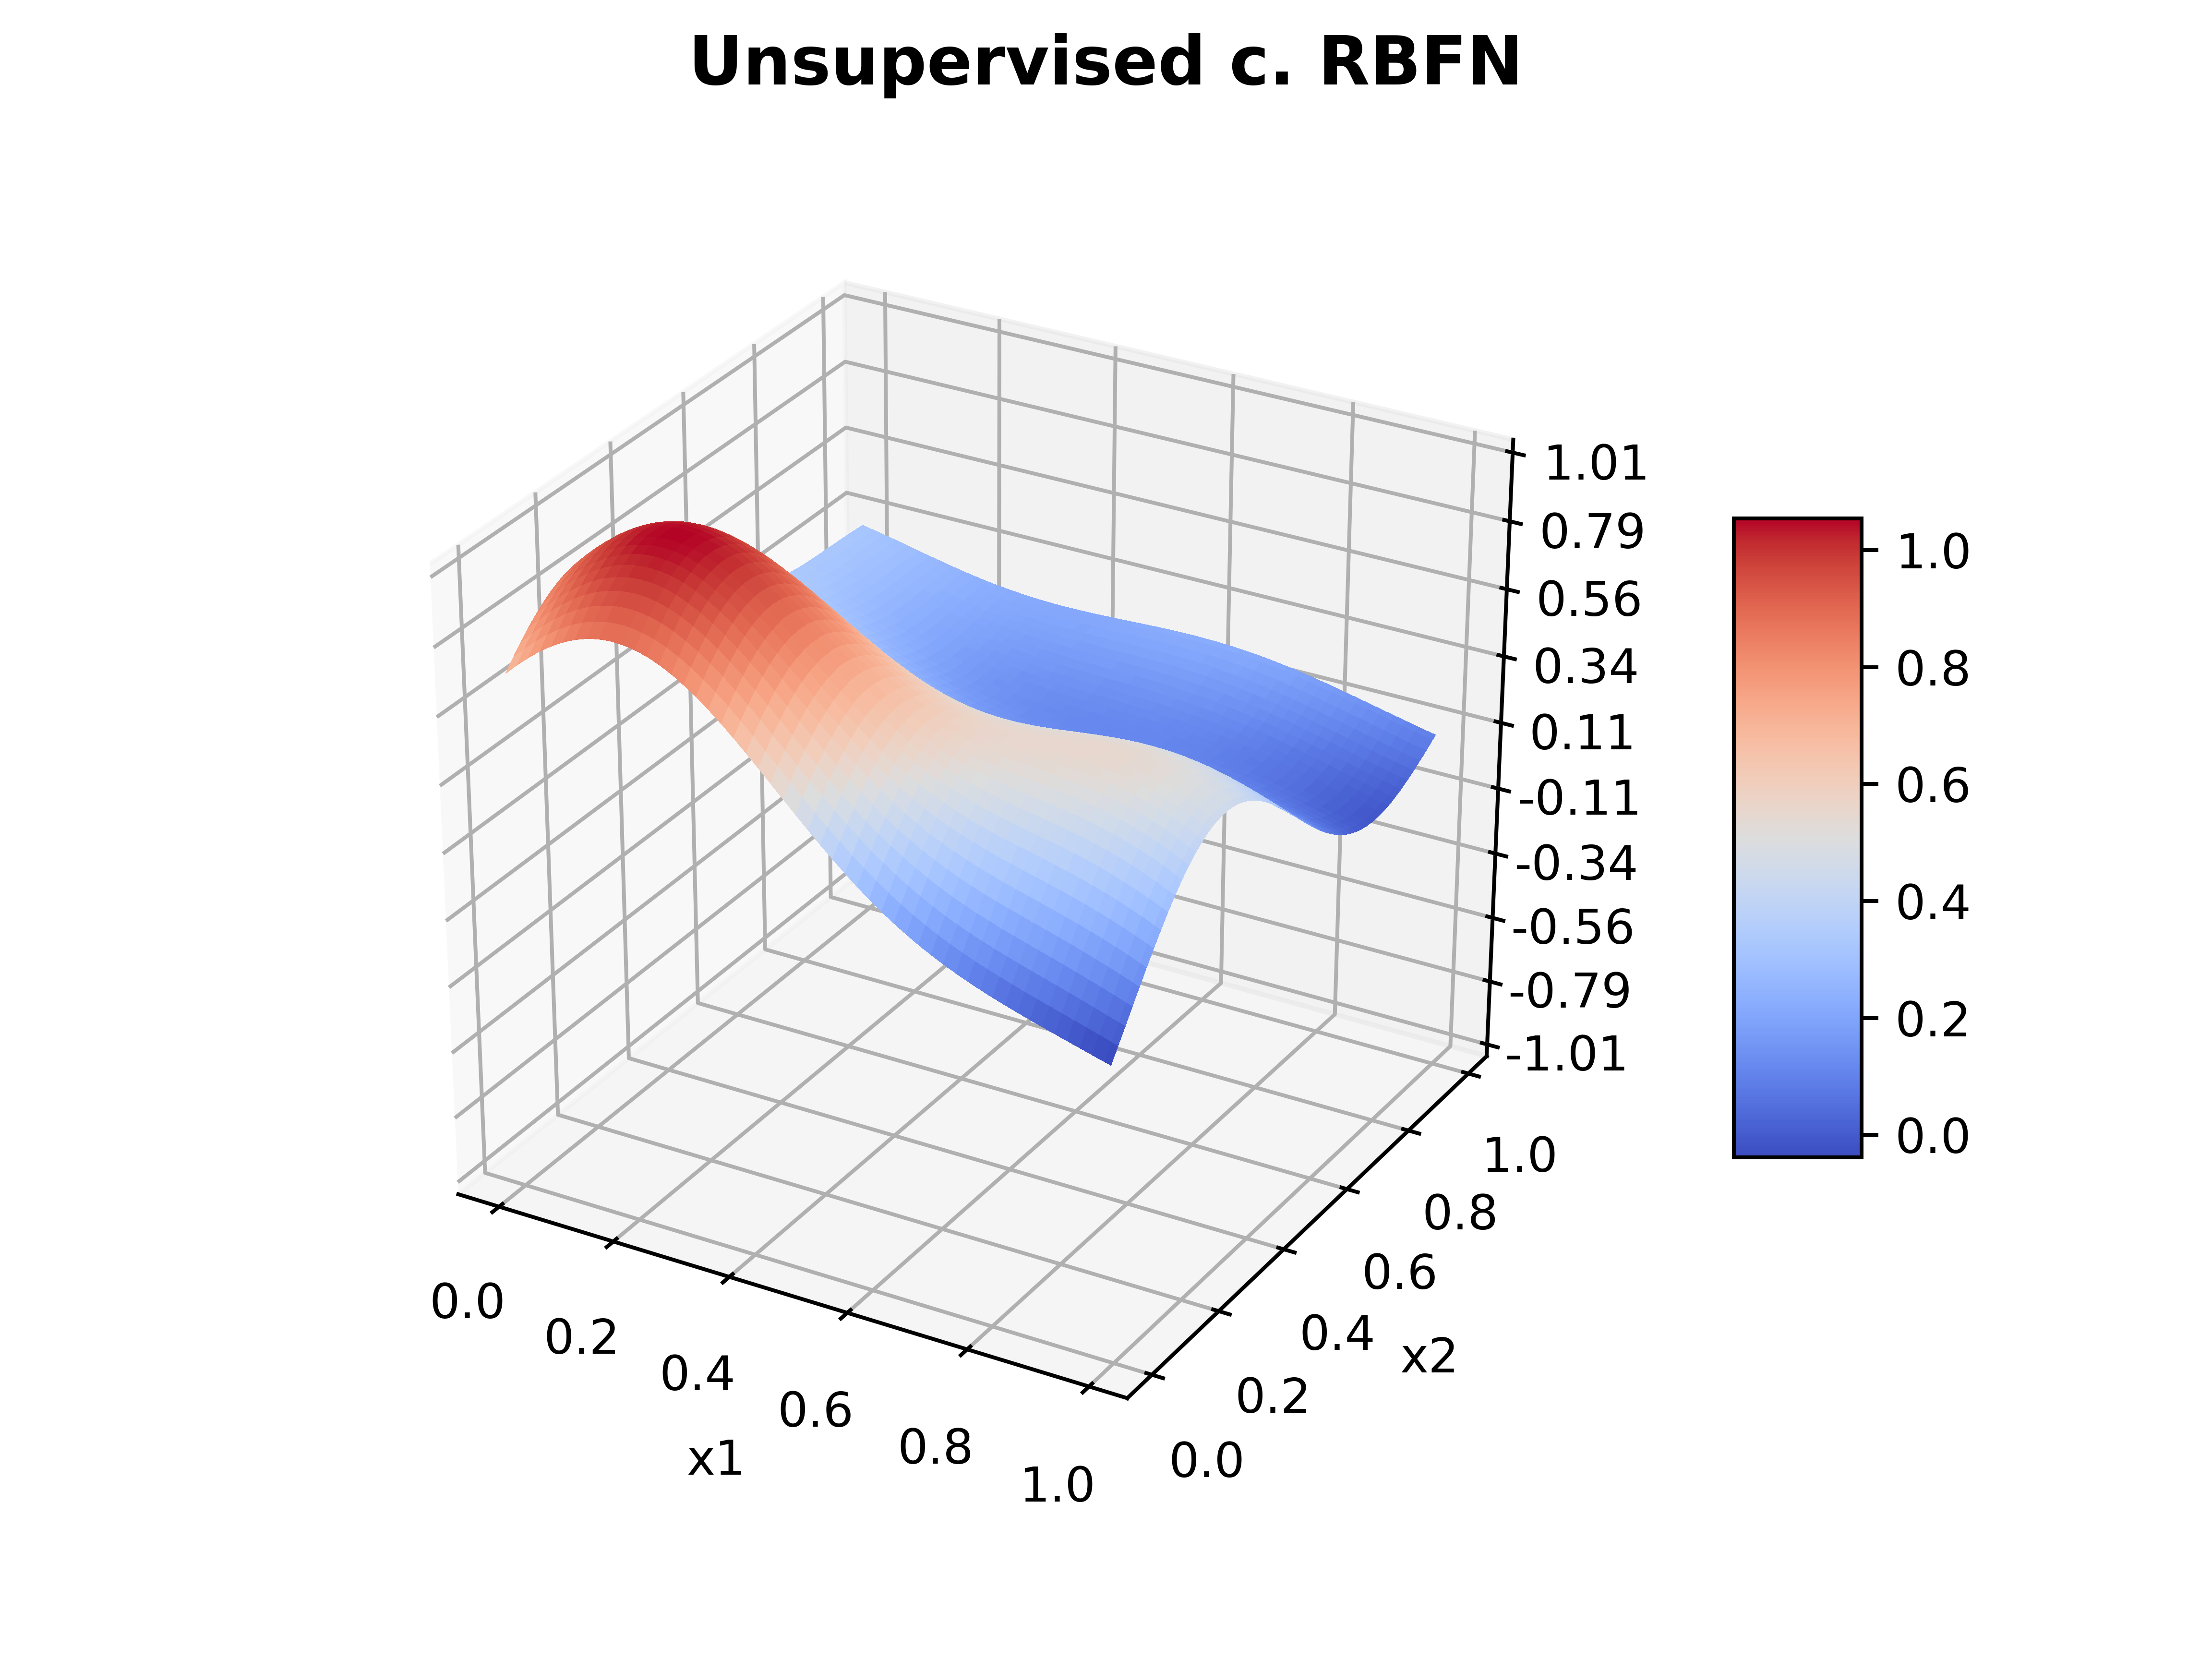
\includegraphics[width=1.0\linewidth]{images/RBFN_Extreme_Learning.png}
	\end{subfigure}
	\caption{In order: the Franke's function and the functions obtained by
		Full MLP, Full RBFN, Extreme MLP, Unisupervised c. RBFN and TBD.
		The hyperparameters used for each network are specified in table
		\ref{tab:experiments}.}
	\label{fig:plots}
\end{figure}

%-------------------------------------------------------------------------------

%\newpage
%\bibliography{bibliography}
%\bibliographystyle{ieeetr}

%-------------------------------------------------------------------------------

\end{document}
\grid
\grid
